\documentclass{beamer}
\usepackage{fontspec}
\usepackage{bibentry}
\setmainfont{Sarasa-Term-SC-Regular}
\setsansfont{HelveticaNeue}
\setmonofont{CascadiaCode}
\setbeamertemplate{frametitle}[default][center]

\mode<presentation> {

% The Beamer class comes with a number of default slide themes
% which change the colors and layouts of slides. Below this is a list
% of all the themes, uncomment each in turn to see what they look like.

\usetheme{default}
%\usetheme{AnnArbor}
%\usetheme{Antibes}
%\usetheme{Bergen}
%\usetheme{Berkeley}
%\usetheme{Berlin}
%\usetheme{Boadilla}
%\usetheme{CambridgeUS}
%\usetheme{Copenhagen}
%\usetheme{Darmstadt}
%\usetheme{Dresden}
%\usetheme{Frankfurt}
%\usetheme{Goettingen}
%\usetheme{Hannover}
%\usetheme{Ilmenau}
%\usetheme{JuanLesPins}
%\usetheme{Luebeck}
%\usetheme{Madrid}
%\usetheme{Malmoe}
%\usetheme{Marburg}
%\usetheme{Montpellier}
%\usetheme{PaloAlto}
%\usetheme{Pittsburgh}
%\usetheme{Rochester}
%\usetheme{Singapore}
%\usetheme{Szeged}
%\usetheme{Warsaw}

% As well as themes, the Beamer class has a number of color themes
% for any slide theme. Uncomment each of these in turn to see how it
% changes the colors of your current slide theme.

%\usecolortheme{albatross}
%\usecolortheme{beaver}
%\usecolortheme{beetle}
%\usecolortheme{crane}
%\usecolortheme{dolphin}
\usecolortheme{dove}
%\usecolortheme{fly}
%\usecolortheme{lily}
%\usecolortheme{orchid}
 %\usecolortheme{rose}
%\usecolortheme{seagull}
%\usecolortheme{seahorse}
%\usecolortheme{whale}
%\usecolortheme{wolverine}

%\setbeamertemplate{footline} % To remove the footer line in all slides uncomment this line
%\setbeamertemplate{footline}[page number] % To replace the footer line in all slides with a simple slide count uncomment this line

%\setbeamertemplate{navigation symbols}{} % To remove the navigation symbols from the bottom of all slides uncomment this line
}

\usepackage{graphicx} % Allows including images
\usepackage{booktabs} % Allows the use of \toprule, \midrule and \bottomrule in tables

%----------------------------------------------------------------------------------------
%	TITLE PAGE
%----------------------------------------------------------------------------------------

\title[Short title]{General Video Game playing AI: A Survey} % The short title appears at the bottom of every slide, the full title is only on the title page

\author{ Wangzhihui Mei 2019124044} % Your name
\institute[JI] % Your institution as it will appear on the bottom of every slide, may be shorthand to save space
{
CCNU-UOW JI \\ % Your institution for the title page
\medskip
\textit{maywzh@gmail.com} % Your email address
}
\date{\today} % Date, can be changed to a custom date

\begin{document}

\begin{frame}
\titlepage % Print the title page as the first slide
\end{frame}

\begin{frame}
\frametitle{Overview} % Table of contents slide, comment this block out to remove it
\tableofcontents % Throughout your presentation, if you choose to use \section{} and \subsection{} commands, these will automatically be printed on this slide as an overview of your presentation
\end{frame}

%----------------------------------------------------------------------------------------
%	PRESENTATION SLIDES
%----------------------------------------------------------------------------------------

%------------------------------------------------
\section{Introduction}
\begin{frame}
\frametitle{Video Game Playing AI}
Video games have long been popular benchmarks for Artificial Intelligence(AI)\cite{1}. Many researches have been done in building a optimal \textbf{Video Game Playing AI(VPAI)}  in certain games. 

Such attempts comprises Chess, Go, Car Racing games, Ms.PacMan, Real-Time Strategy (RTS) games and Super Mario Bros, etc. 
\end{frame}

\subsection{Research Scope}
\begin{frame}
  \frametitle{Research Scope}
  In this research, we focus on \textbf{General Video Game Playing AI(GVPAI)}.

  GVPAI aims at building an no-human-intervening game-playing agent that is able to playing multiple games rather than specialized VPAI designed for certain one game\cite{1}.

\end{frame}

\subsection{Motivation}
\begin{frame}
  \frametitle{Motivation\cite{2}}
  The objective of General Video Game Playing (GVGP) is to by-pass the addition of game specific knowledge, especially if the algorithm is tested in games that have not been played before.

  Obviously, algorithms that approach GVGP problems may still count on some kind of domain knowledge, and the questions raised above could still be asked. Indeed, many different algorithms can be employed for GVGP, and chances are that heuristics will still make a big difference. 
  
  However, by reducing the game-dependent knowledge, approaches are forced to be more general, and research conducted in this field is closer to the open domain of General Artificial Intelligence.
  
\end{frame}



%------------------------------------------------
\section{Landscapes}
\begin{frame}
\frametitle{Landscapes of GVPAI}
\begin{itemize}
\item Knowledge Representation
\item Search
\item Planning
\item Learning
\item Generality
\end{itemize}
\end{frame}

%------------------------------------------------
%[General general game AI]
\subsection{Knowledge Representation}
\begin{frame}
\frametitle{Knowledge Representation and Reasoning\cite{3}}
GVPAI requires a formal, symbolic language in which the rules of arbitrary games can be described to a system. The general Game Description Language (GDL) has been developed for that purpose. There are several challenging reasoning problems.
\begin{itemize}
  \item Reasoning about actions
  \item Automated theorem proving
  \item Other KRR techniques
\end{itemize}
\end{frame}

\subsection{Search}
\begin{frame}
  \frametitle{Search\cite{12}}
  Once a GVPAI system is capable of computing legal moves and position updates from the game rules, it can search through the space of pos- sible ways in which the game can proceed
  \begin{itemize}
    \item Monte Carlo Tree Search
    \item Informed search -- Uses problem-specific knowledge.
  \end{itemize}

\end{frame}

\subsection{Planning}
\begin{frame}
  \frametitle{Planning}
  Planning is closely related to GVGP, as both are instances of general problem solving, where the specifics of a problem are unknown until runtime.
\end{frame}

\subsection{Learning}
\begin{frame}
  \frametitle{Learning}
  The very idea of general game playing is to build systems that automatically learn to master arbitrary new games.
  

\end{frame}
%------------------------------------------------

%------------------------------------------------
\subsection{Generality}
\begin{frame}
\frametitle{Generality\cite{4}}
\begin{columns}[c] % The "c" option specifies centered vertical alignment while the "t" option is used for top vertical alignment

\column{.45\textwidth} % Left column and width
\textbf{Heading}
\begin{enumerate}
\item Game generality
\item Task generality
\item Player generality 
\end{enumerate}


\column{.5\textwidth} % Right column and width
Develop AI methods that work with not just one game, but with multiple game.

Develop methods that can do not only one task but several differnet related tasks.

Develop methods that can model, respond or reproduce the large variability among humans in design style, playing style, preferences and abilities.
\end{columns}
\end{frame}

\section{Approachs}
\begin{frame}
  \frametitle{Approachs}
  \begin{itemize}
    \item Neural Network(NN)
    \item Reinforcement Learning(RL)
    \item Monte-Carlo Tree Search(MCTS)
  \end{itemize}
\end{frame}


\subsection{Neural Network}
\begin{frame}
\frametitle{NN-based GVGP}
M. Hausknecht et al. \cite{5} employed evolutionary neural networks to extract higher-dimensional representation forms from the raw game screen.

All algorithms encode Artificial Neural Networks (ANNs) which are represented by weights and connectivity(topology).
\begin{figure}
  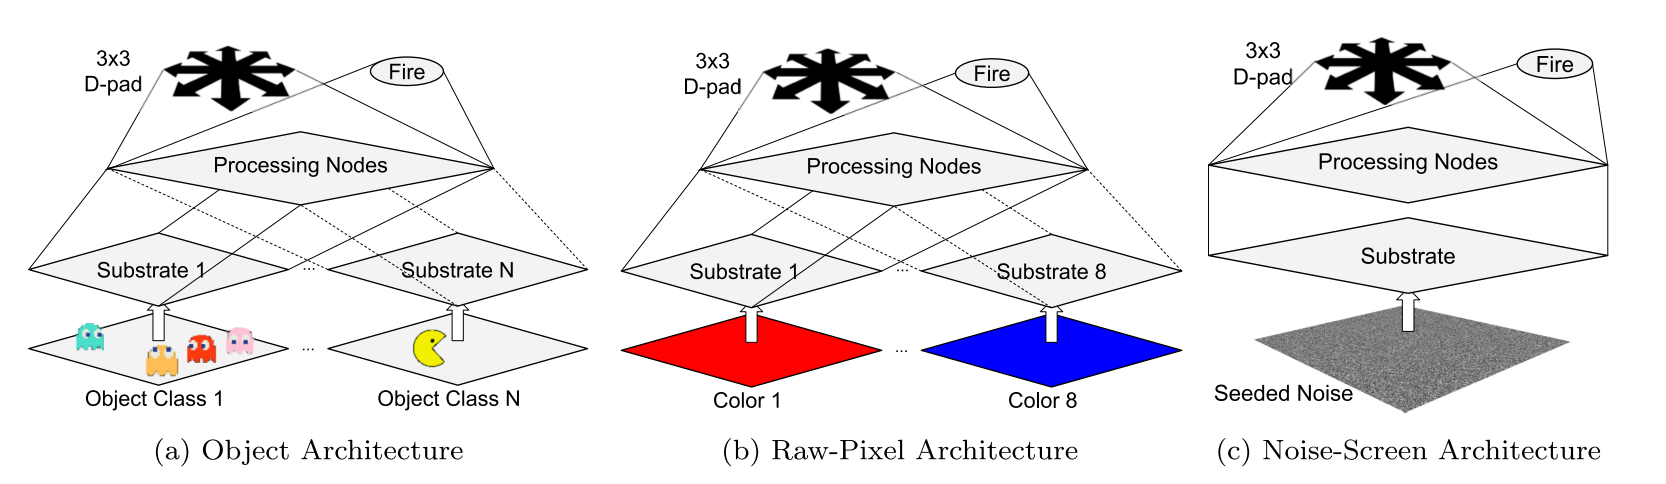
\includegraphics[width=1\linewidth]{figures/m1p1}
  \caption{ANN topology for 3 different state representation}
\end{figure}
\end{frame}

\subsection{Reinforcement Learning}
\begin{frame}[allowframebreaks]
\frametitle{RL-based GVGP}
Yavar Naddaf \cite{6} used 2 main approaches: RL-based and search-based methods. RL-based methods use feature vectors generated from the game screen as well as the console RAM to learn to play a given game. The search-based methods use the emulator to simulate the consequence of actions into the future, aiming to play as well as possible by only exploring a very small fraction of the state-space.

\begin{figure}
  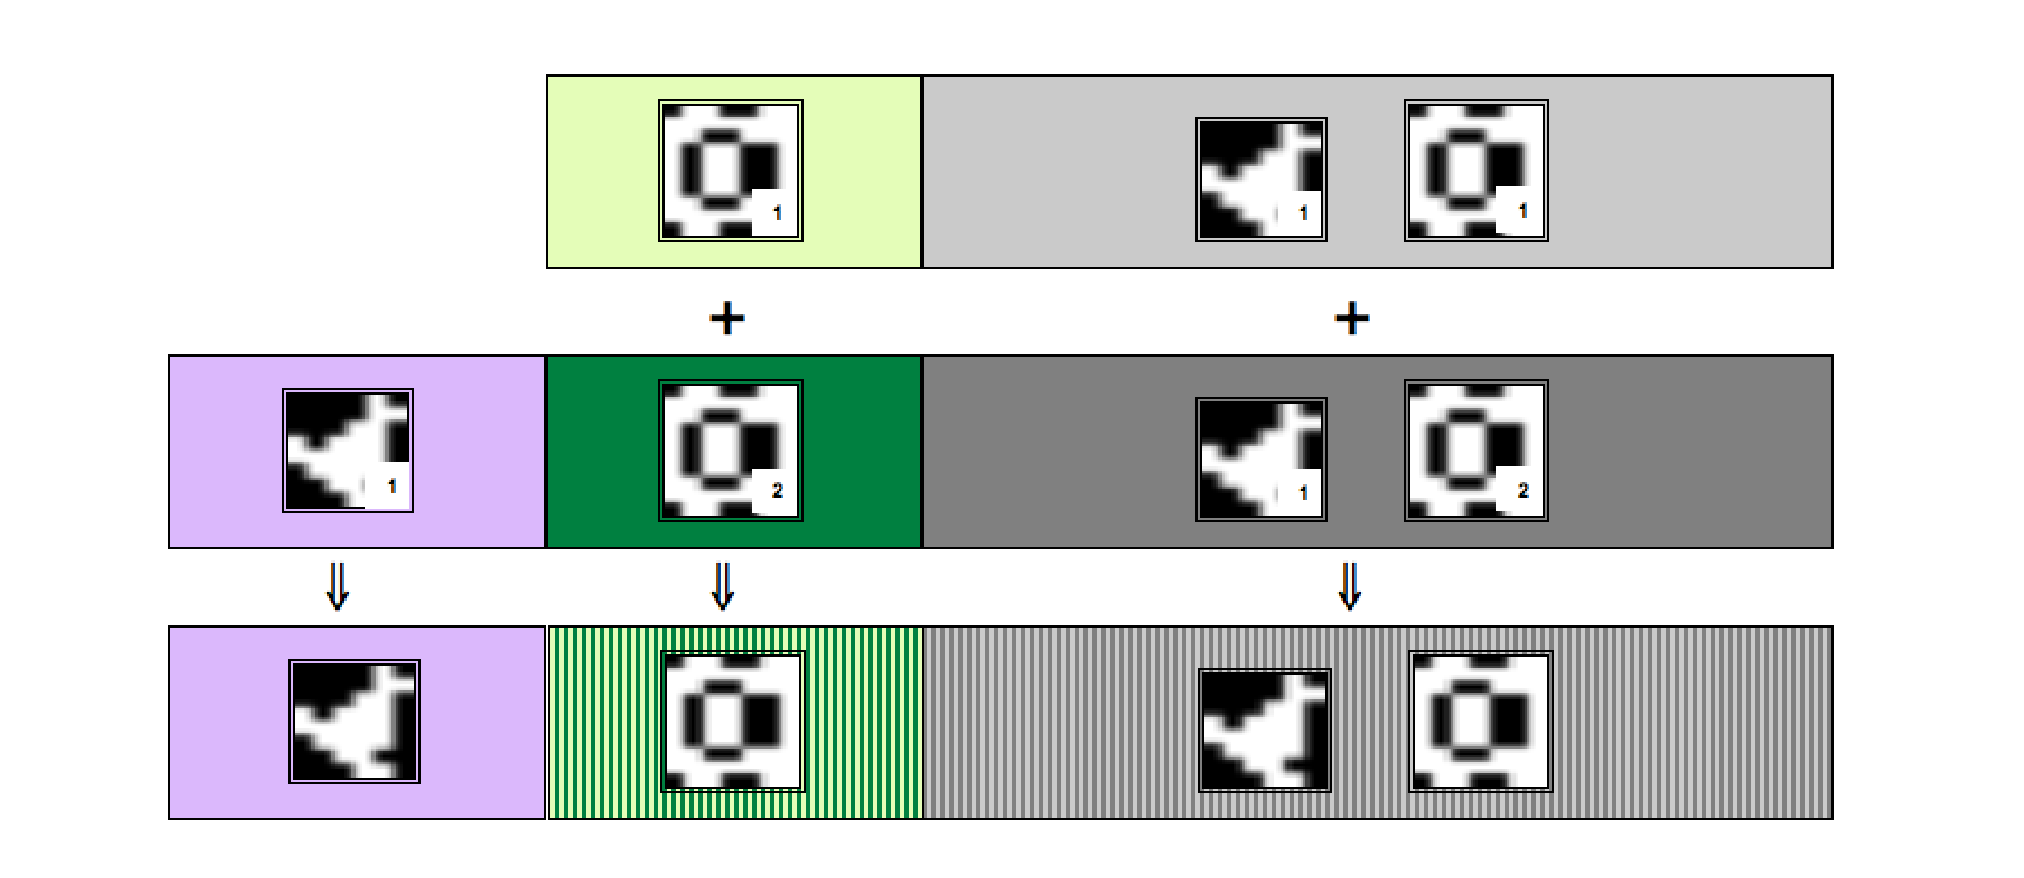
\includegraphics[width=0.6\linewidth]{figures/featurevector}
  \caption{ Conceptual figure of feature vector generation for the game Freeway}
\end{figure}

Bellemare et al. \cite{7} explored the concept of contingency awareness (the recognition that a future observation is under an agent's control and not solely determined by the environment) using Atari 2600 games.

The research introduced a technique for accurately identifying contingent regions and describe how to exploit this knowledge to generate improved features for value function approximation.
\begin{figure}
  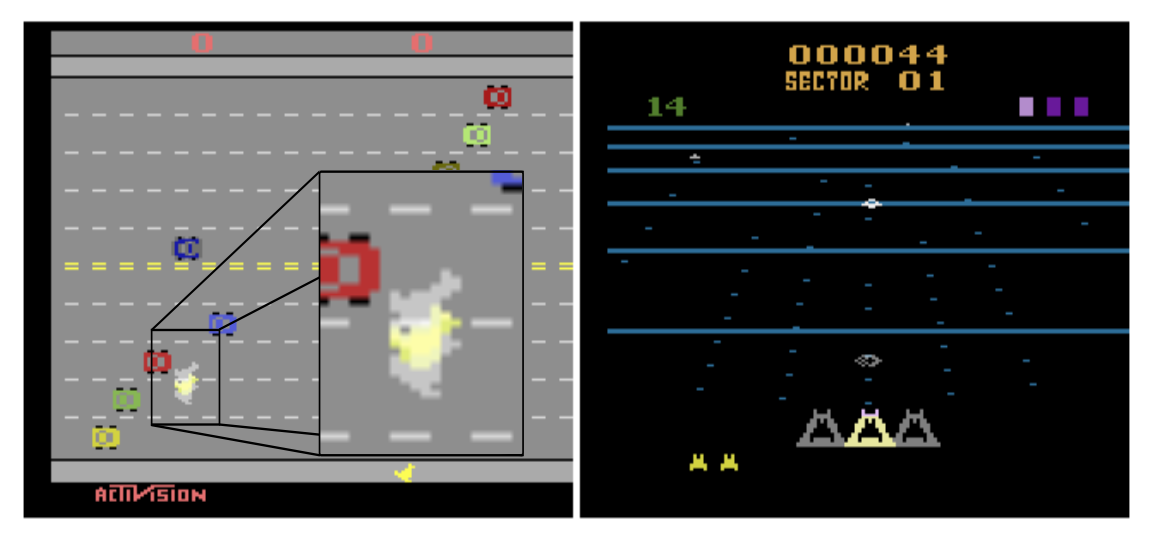
\includegraphics[width=0.5\linewidth]{figures/contingentregions}
  \caption{ The contingent regions, shown by a transparent overlay, for Freeway (left) and Beam Rider (right)}
\end{figure}
\end{frame}

\subsection{Monte-Carlo Tree Search}
\begin{frame}[allowframebreaks]
\frametitle{MCTS-based GVGP}
Perez et. al. \cite{8} explored the performance of a vanilla Monte Carlo Tree Search algorithm, and analyzed the main difficulties encountered when tackling this kind of scenarios and did some modifications to overcome these issues, strengthening the algorithm's ability to gather and discover knowledge, and taking advantage of past experiences.

\begin{figure}[c]
  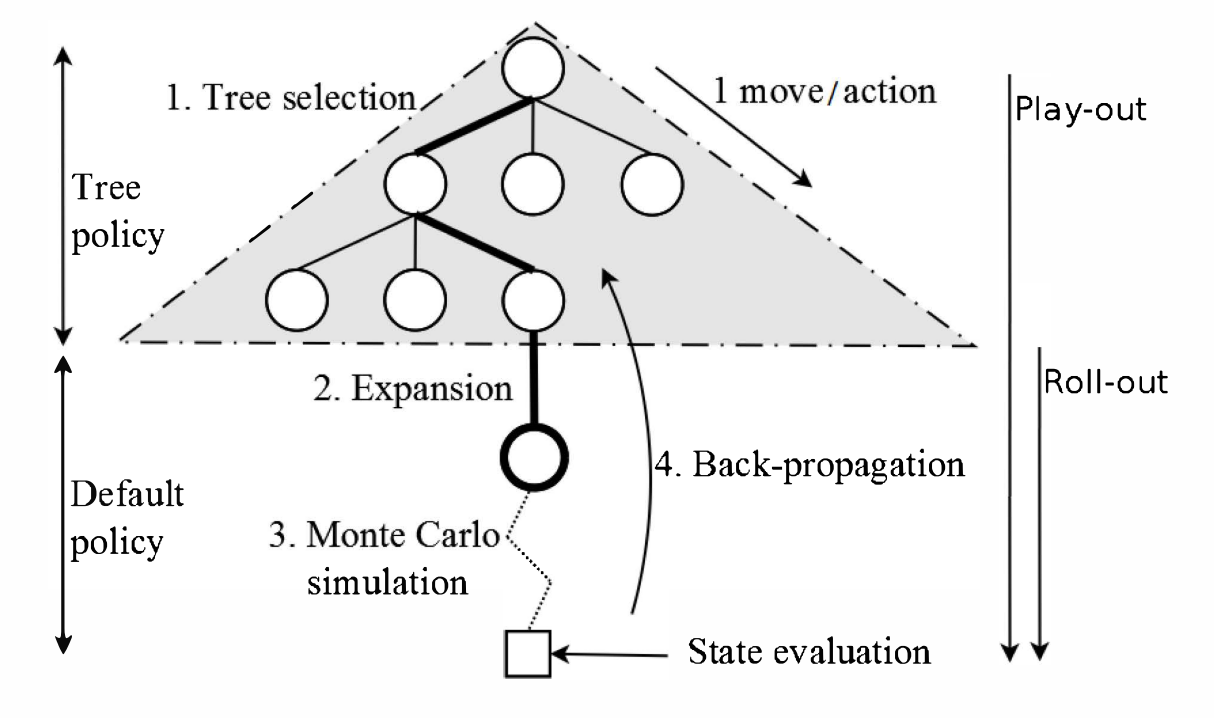
\includegraphics[width=0.6\linewidth]{figures/mctskb}
  \caption{ MCTS algorithm steps }
\end{figure}

Park and Kim\cite{9} propose to use influence map (IM) to solve
the MCTS’s horizon effect problem.

\begin{figure}[c]
  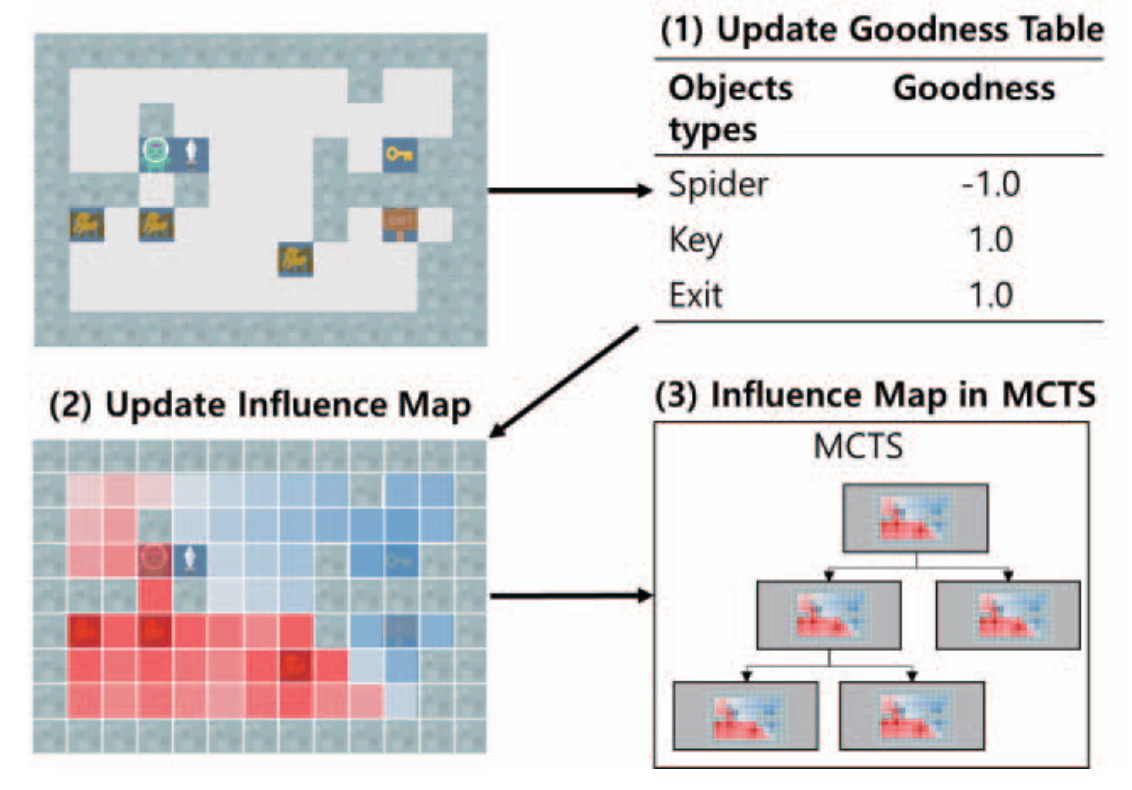
\includegraphics[width=0.6\linewidth]{figures/kim}
  \caption{ Overview of proposed method (blue is good influence and red is bad influence) }
\end{figure}

Sironi et.al.\cite{10} designed three Self-Adaptive MCTS (SA-MCTS) agents that optimize the parameters of a standard non-Self-Adaptive MCTS agent of GVPAI. 

The three agents select the parameter values using Naive Monte-Carlo, an Evolutionary Algorithm and an N-Tuple Bandit Evolutionary Algorithm respectively, and are tested on 20 single-player games.

\begin{figure}[c]
  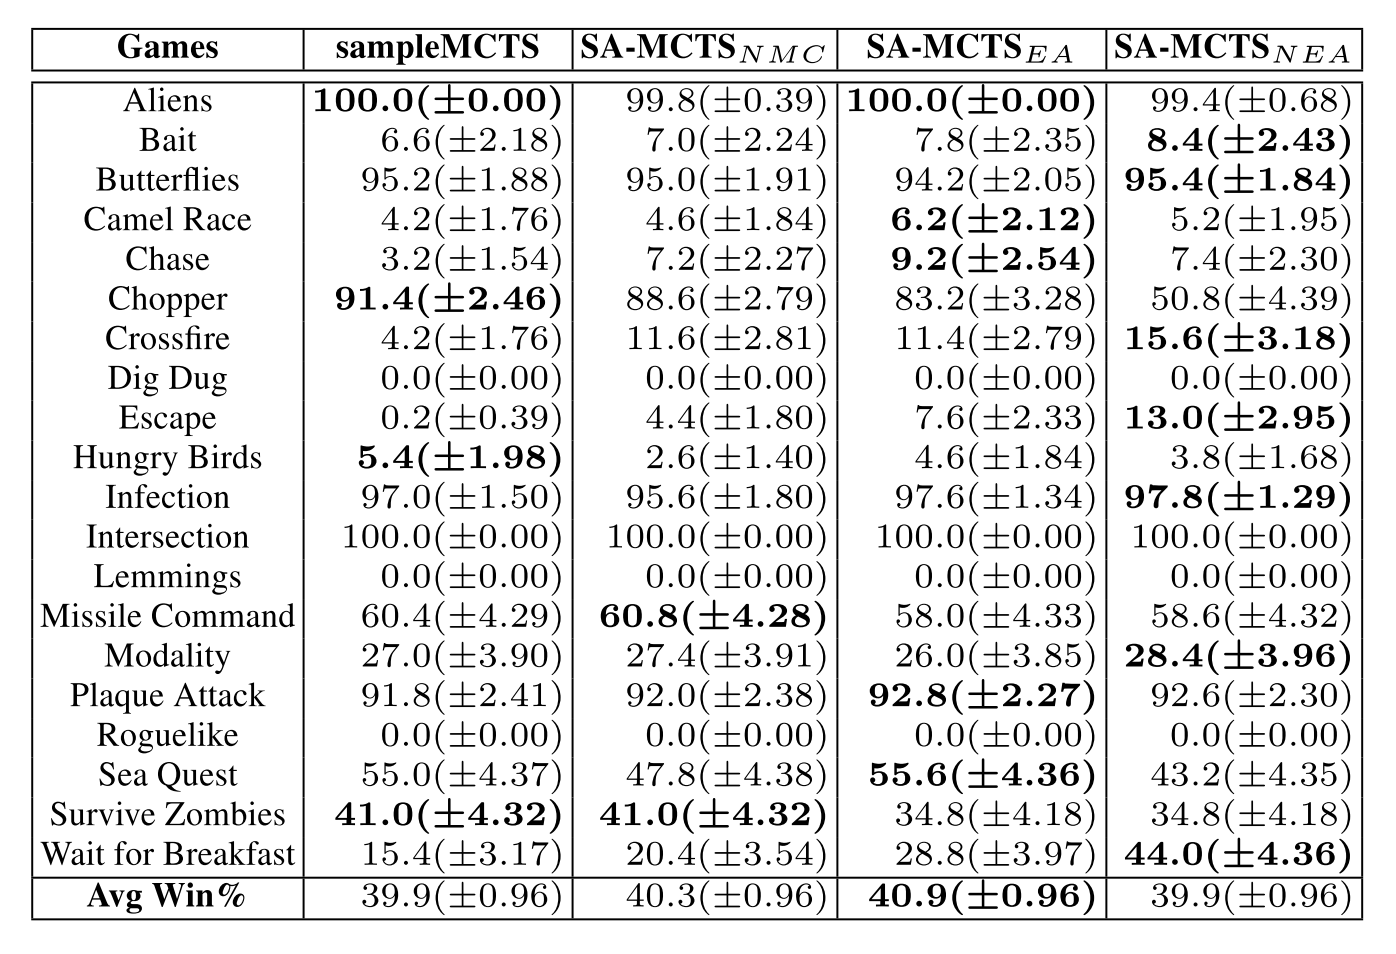
\includegraphics[width=1\linewidth]{figures/figure1}
  \caption{ Average win rate over 5 levels of each game}
\end{figure}
\end{frame}

\section{Conclusion}
\begin{frame}
  \frametitle{Conclusion}
  General game playing is an exciting, still young but on the verge of maturing topic, which touches upon a broad range of aspects of artificial intelligence. it provides a rich source of interesting and challenging problems for many an AI researcher.
  

\end{frame}


\begin{frame}[allowframebreaks]
\frametitle{References}
\footnotesize{
\begin{thebibliography}{99} % Beamer does not support BibTeX so references must be inserted manually as below
    \bibitem{1}
    Perez-Liebana, D., Samothrakis, S., Togelius, J., Lucas, S. M., \& Schaul, T. (2016). 
    \newblock General video game AI: Competition, challenges, and opportunities. 
    \newblock In 30th AAAI Conference on Artificial Intelligence, AAAI 2016, 4335–4337.

    \bibitem{2}
    Perez, D., Samothrakis, S., \& Lucas, S. (2014). 
    \newblock Knowledge-based fast evolutionary MCTS for general video game playing.
    \newblock IEEE Conference on Computatonal Intelligence and Games, CIG, 1–8.


    \bibitem{3}
    Yannakakis, G. N. (2012). 
    \newblock Game AI revisited.
    \newblock In CF ’12 - Proceedings of the ACM Computing Frontiers Conference, 285–292.

    \bibitem{4}
    Togelius, J., \& Yannakakis, G. N. (2016). 
    \newblock General general game AI. 
    \newblock In IEEE Conference on Computatonal Intelligence and Games, CIG, 0, 1–8.

    \bibitem{5}
    Hausknecht, M., Lehman, J., Miikkulainen, R., \& Stone, P. (2014). 
    \newblock A neuroevolution approach to general atari game playing. 
    \newblock In IEEE Transactions on Computational Intelligence and AI in Games, 6(4), 355–366.

    \bibitem{6}
    Naddaf, Y. (2010). 
    \newblock Game-independent AI agents for playing Atari 2600 console games.
    \newblock In ProQuest Dissertations and Theses, MR60546, 79.

    \bibitem{7}
    Bellemare, M. G., Veness, J., \& Bowling, M. (2012). 
    \newblock Investigating contingency awareness using Atari 2600 games. 
    \newblock In Proceedings of the National Conference on Artificial Intelligence, 2, 864–871.

    \bibitem{8}
    Perez, D., Samothrakis, S., \& Lucas, S. (2014).
    \newblock Knowledge-based fast evolutionary MCTS for general video game playing. 
    \newblock In IEEE Conference on Computatonal Intelligence and Games, CIG, 1–8.

    \bibitem{9}
    Park, H., \& Kim, K. J. (2015). 
    \newblock MCTS with influence map for general video game playing. 
    \newblock In 2015 IEEE Conference on Computational Intelligence and Games, CIG 2015 - Proceedings, 534–535.

    \bibitem{10}
    Sironi, C. F., Liu, J., Perez-Liebana, D., Gaina, R. D., Bravi, I., Lucas, S. M., \& Winands, M. H. M. (2018). 
    \newblock Self-adaptive MCTS for General Video Game Playing. 
    \newblock In Lecture Notes in Computer Science (Including Subseries Lecture Notes in Artificial Intelligence and Lecture Notes in Bioinformatics), 10784 LNCS(January), 358–375.

    \bibitem{11}
    Mendes, A., Togelius, J., \& Nealen, A. (2016). 
    \newblock Hyper-heuristic general video game playing. 
    \newblock In IEEE Conference on Computatonal Intelligence and Games, CIG, 0, 1–8.

    \bibitem{12}
    Thielscher, M. (2011). 
    \newblock General game playing in AI research and education. 
    \newblock In Lecture Notes in Computer Science (Including Subseries Lecture Notes in Artificial Intelligence and Lecture Notes in Bioinformatics), 7006 LNAI, 26–37.

    \end{thebibliography}
}
\end{frame}

%------------------------------------------------

\begin{frame}
\Huge{\centerline{The End}}
\end{frame}

%----------------------------------------------------------------------------------------

\end{document} 